% Graphic for TeX using PGF
% Title: /home/tobias/Documents/Studium/softwareengineering/organisation/documentations/softwareentwurf/uml-diagramms/Flowchart-MainLoop.dia
% Creator: Dia v0.97.2
% CreationDate: Sun Oct 18 16:55:48 2015
% For: tobias
% \usepackage{tikz}
% The following commands are not supported in PSTricks at present
% We define them conditionally, so when they are implemented,
% this pgf file will use them.
\ifx\du\undefined
  \newlength{\du}
\fi
\setlength{\du}{15\unitlength}
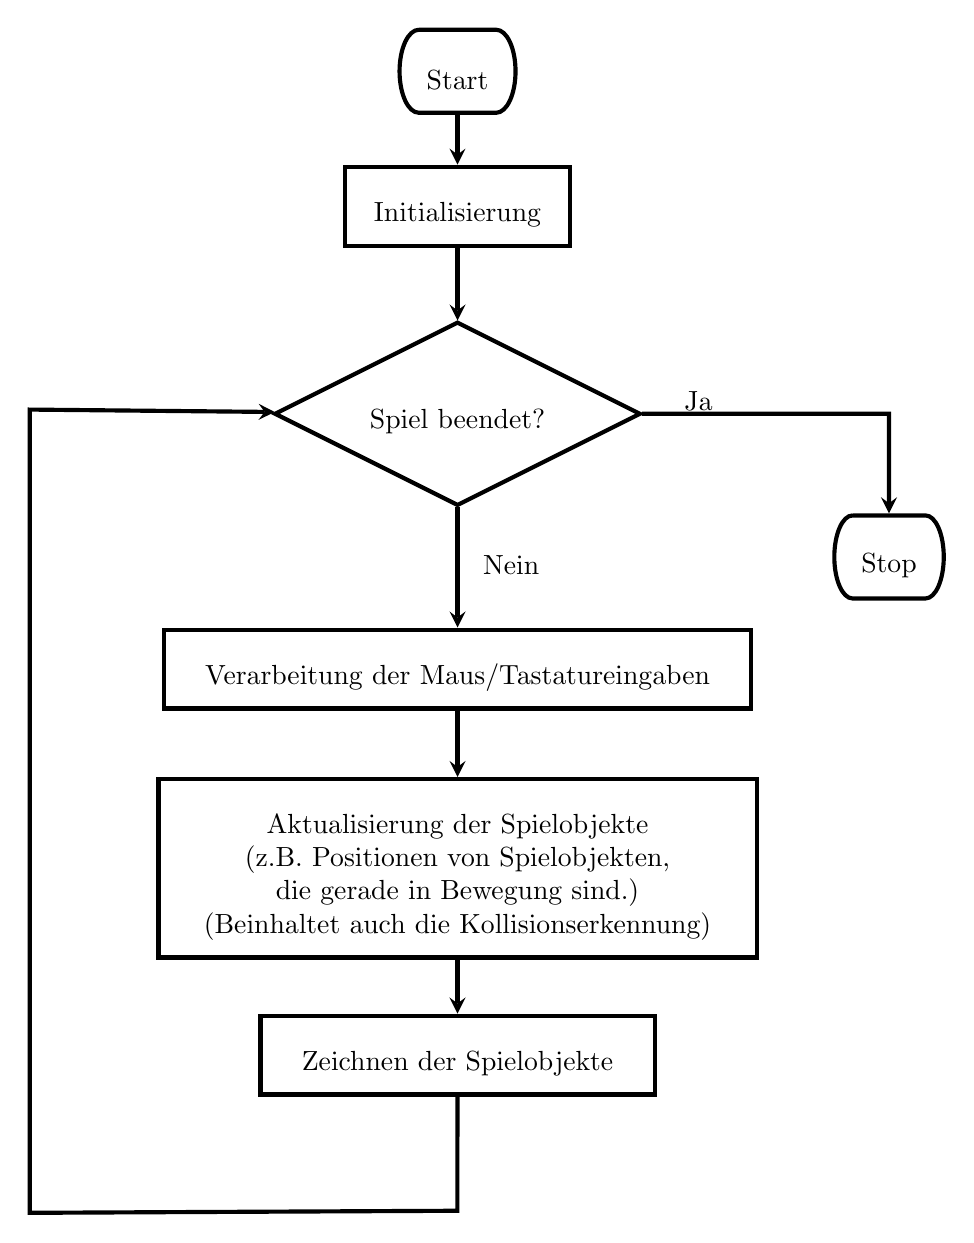
\begin{tikzpicture}
\pgftransformxscale{1.000000}
\pgftransformyscale{-1.000000}
\definecolor{dialinecolor}{rgb}{0.000000, 0.000000, 0.000000}
\pgfsetstrokecolor{dialinecolor}
\definecolor{dialinecolor}{rgb}{1.000000, 1.000000, 1.000000}
\pgfsetfillcolor{dialinecolor}
\pgfsetlinewidth{0.100000\du}
\pgfsetdash{}{0pt}
\pgfsetdash{}{0pt}
\pgfsetbuttcap
\pgfsetmiterjoin
\pgfsetlinewidth{0.100000\du}
\pgfsetbuttcap
\pgfsetmiterjoin
\pgfsetdash{}{0pt}
\definecolor{dialinecolor}{rgb}{1.000000, 1.000000, 1.000000}
\pgfsetfillcolor{dialinecolor}
\pgfpathmoveto{\pgfpoint{22.223750\du}{6.200000\du}}
\pgfpathlineto{\pgfpoint{24.086250\du}{6.200000\du}}
\pgfpathcurveto{\pgfpoint{24.343408\du}{6.200000\du}}{\pgfpoint{24.551875\du}{6.647715\du}}{\pgfpoint{24.551875\du}{7.200000\du}}
\pgfpathcurveto{\pgfpoint{24.551875\du}{7.752285\du}}{\pgfpoint{24.343408\du}{8.200000\du}}{\pgfpoint{24.086250\du}{8.200000\du}}
\pgfpathlineto{\pgfpoint{22.223750\du}{8.200000\du}}
\pgfpathcurveto{\pgfpoint{21.966592\du}{8.200000\du}}{\pgfpoint{21.758125\du}{7.752285\du}}{\pgfpoint{21.758125\du}{7.200000\du}}
\pgfpathcurveto{\pgfpoint{21.758125\du}{6.647715\du}}{\pgfpoint{21.966592\du}{6.200000\du}}{\pgfpoint{22.223750\du}{6.200000\du}}
\pgfusepath{fill}
\definecolor{dialinecolor}{rgb}{0.000000, 0.000000, 0.000000}
\pgfsetstrokecolor{dialinecolor}
\pgfpathmoveto{\pgfpoint{22.223750\du}{6.200000\du}}
\pgfpathlineto{\pgfpoint{24.086250\du}{6.200000\du}}
\pgfpathcurveto{\pgfpoint{24.343408\du}{6.200000\du}}{\pgfpoint{24.551875\du}{6.647715\du}}{\pgfpoint{24.551875\du}{7.200000\du}}
\pgfpathcurveto{\pgfpoint{24.551875\du}{7.752285\du}}{\pgfpoint{24.343408\du}{8.200000\du}}{\pgfpoint{24.086250\du}{8.200000\du}}
\pgfpathlineto{\pgfpoint{22.223750\du}{8.200000\du}}
\pgfpathcurveto{\pgfpoint{21.966592\du}{8.200000\du}}{\pgfpoint{21.758125\du}{7.752285\du}}{\pgfpoint{21.758125\du}{7.200000\du}}
\pgfpathcurveto{\pgfpoint{21.758125\du}{6.647715\du}}{\pgfpoint{21.966592\du}{6.200000\du}}{\pgfpoint{22.223750\du}{6.200000\du}}
\pgfusepath{stroke}
% setfont left to latex
\definecolor{dialinecolor}{rgb}{0.000000, 0.000000, 0.000000}
\pgfsetstrokecolor{dialinecolor}
\node at (23.155000\du,7.400000\du){Start};
\pgfsetlinewidth{0.100000\du}
\pgfsetdash{}{0pt}
\pgfsetdash{}{0pt}
\pgfsetbuttcap
\pgfsetmiterjoin
\pgfsetlinewidth{0.100000\du}
\pgfsetbuttcap
\pgfsetmiterjoin
\pgfsetdash{}{0pt}
\definecolor{dialinecolor}{rgb}{1.000000, 1.000000, 1.000000}
\pgfsetfillcolor{dialinecolor}
\pgfpathmoveto{\pgfpoint{32.671250\du}{17.900000\du}}
\pgfpathlineto{\pgfpoint{34.428750\du}{17.900000\du}}
\pgfpathcurveto{\pgfpoint{34.671410\du}{17.900000\du}}{\pgfpoint{34.868125\du}{18.347715\du}}{\pgfpoint{34.868125\du}{18.900000\du}}
\pgfpathcurveto{\pgfpoint{34.868125\du}{19.452285\du}}{\pgfpoint{34.671410\du}{19.900000\du}}{\pgfpoint{34.428750\du}{19.900000\du}}
\pgfpathlineto{\pgfpoint{32.671250\du}{19.900000\du}}
\pgfpathcurveto{\pgfpoint{32.428590\du}{19.900000\du}}{\pgfpoint{32.231875\du}{19.452285\du}}{\pgfpoint{32.231875\du}{18.900000\du}}
\pgfpathcurveto{\pgfpoint{32.231875\du}{18.347715\du}}{\pgfpoint{32.428590\du}{17.900000\du}}{\pgfpoint{32.671250\du}{17.900000\du}}
\pgfusepath{fill}
\definecolor{dialinecolor}{rgb}{0.000000, 0.000000, 0.000000}
\pgfsetstrokecolor{dialinecolor}
\pgfpathmoveto{\pgfpoint{32.671250\du}{17.900000\du}}
\pgfpathlineto{\pgfpoint{34.428750\du}{17.900000\du}}
\pgfpathcurveto{\pgfpoint{34.671410\du}{17.900000\du}}{\pgfpoint{34.868125\du}{18.347715\du}}{\pgfpoint{34.868125\du}{18.900000\du}}
\pgfpathcurveto{\pgfpoint{34.868125\du}{19.452285\du}}{\pgfpoint{34.671410\du}{19.900000\du}}{\pgfpoint{34.428750\du}{19.900000\du}}
\pgfpathlineto{\pgfpoint{32.671250\du}{19.900000\du}}
\pgfpathcurveto{\pgfpoint{32.428590\du}{19.900000\du}}{\pgfpoint{32.231875\du}{19.452285\du}}{\pgfpoint{32.231875\du}{18.900000\du}}
\pgfpathcurveto{\pgfpoint{32.231875\du}{18.347715\du}}{\pgfpoint{32.428590\du}{17.900000\du}}{\pgfpoint{32.671250\du}{17.900000\du}}
\pgfusepath{stroke}
% setfont left to latex
\definecolor{dialinecolor}{rgb}{0.000000, 0.000000, 0.000000}
\pgfsetstrokecolor{dialinecolor}
\node at (33.550000\du,19.100000\du){Stop};
\definecolor{dialinecolor}{rgb}{1.000000, 1.000000, 1.000000}
\pgfsetfillcolor{dialinecolor}
\fill (23.155000\du,13.255511\du)--(27.546910\du,15.451466\du)--(23.155000\du,17.647421\du)--(18.763090\du,15.451466\du)--cycle;
\pgfsetlinewidth{0.100000\du}
\pgfsetdash{}{0pt}
\pgfsetdash{}{0pt}
\pgfsetmiterjoin
\definecolor{dialinecolor}{rgb}{0.000000, 0.000000, 0.000000}
\pgfsetstrokecolor{dialinecolor}
\draw (23.155000\du,13.255511\du)--(27.546910\du,15.451466\du)--(23.155000\du,17.647421\du)--(18.763090\du,15.451466\du)--cycle;
% setfont left to latex
\definecolor{dialinecolor}{rgb}{0.000000, 0.000000, 0.000000}
\pgfsetstrokecolor{dialinecolor}
\node at (23.155000\du,15.646466\du){Spiel beendet?};
\definecolor{dialinecolor}{rgb}{1.000000, 1.000000, 1.000000}
\pgfsetfillcolor{dialinecolor}
\fill (20.438750\du,9.500449\du)--(20.438750\du,11.400449\du)--(25.871250\du,11.400449\du)--(25.871250\du,9.500449\du)--cycle;
\pgfsetlinewidth{0.100000\du}
\pgfsetdash{}{0pt}
\pgfsetdash{}{0pt}
\pgfsetmiterjoin
\definecolor{dialinecolor}{rgb}{0.000000, 0.000000, 0.000000}
\pgfsetstrokecolor{dialinecolor}
\draw (20.438750\du,9.500449\du)--(20.438750\du,11.400449\du)--(25.871250\du,11.400449\du)--(25.871250\du,9.500449\du)--cycle;
% setfont left to latex
\definecolor{dialinecolor}{rgb}{0.000000, 0.000000, 0.000000}
\pgfsetstrokecolor{dialinecolor}
\node at (23.155000\du,10.645449\du){Initialisierung};
\pgfsetlinewidth{0.100000\du}
\pgfsetdash{}{0pt}
\pgfsetdash{}{0pt}
\pgfsetbuttcap
{
\definecolor{dialinecolor}{rgb}{0.000000, 0.000000, 0.000000}
\pgfsetfillcolor{dialinecolor}
% was here!!!
\pgfsetarrowsend{stealth}
\definecolor{dialinecolor}{rgb}{0.000000, 0.000000, 0.000000}
\pgfsetstrokecolor{dialinecolor}
\draw (23.155000\du,8.249095\du)--(23.155000\du,9.450158\du);
}
% setfont left to latex
\definecolor{dialinecolor}{rgb}{0.000000, 0.000000, 0.000000}
\pgfsetstrokecolor{dialinecolor}
\node[anchor=west] at (28.350000\du,15.150000\du){Ja};
\pgfsetlinewidth{0.100000\du}
\pgfsetdash{}{0pt}
\pgfsetdash{}{0pt}
\pgfsetbuttcap
{
\definecolor{dialinecolor}{rgb}{0.000000, 0.000000, 0.000000}
\pgfsetfillcolor{dialinecolor}
% was here!!!
\pgfsetarrowsend{stealth}
\definecolor{dialinecolor}{rgb}{0.000000, 0.000000, 0.000000}
\pgfsetstrokecolor{dialinecolor}
\draw (23.155000\du,11.450714\du)--(23.155000\du,13.205511\du);
}
\definecolor{dialinecolor}{rgb}{1.000000, 1.000000, 1.000000}
\pgfsetfillcolor{dialinecolor}
\fill (16.077500\du,20.651409\du)--(16.077500\du,22.551409\du)--(30.232500\du,22.551409\du)--(30.232500\du,20.651409\du)--cycle;
\pgfsetlinewidth{0.100000\du}
\pgfsetdash{}{0pt}
\pgfsetdash{}{0pt}
\pgfsetmiterjoin
\definecolor{dialinecolor}{rgb}{0.000000, 0.000000, 0.000000}
\pgfsetstrokecolor{dialinecolor}
\draw (16.077500\du,20.651409\du)--(16.077500\du,22.551409\du)--(30.232500\du,22.551409\du)--(30.232500\du,20.651409\du)--cycle;
% setfont left to latex
\definecolor{dialinecolor}{rgb}{0.000000, 0.000000, 0.000000}
\pgfsetstrokecolor{dialinecolor}
\node at (23.155000\du,21.796409\du){Verarbeitung der Maus/Tastatureingaben};
\pgfsetlinewidth{0.100000\du}
\pgfsetdash{}{0pt}
\pgfsetdash{}{0pt}
\pgfsetbuttcap
{
\definecolor{dialinecolor}{rgb}{0.000000, 0.000000, 0.000000}
\pgfsetfillcolor{dialinecolor}
% was here!!!
\pgfsetarrowsend{stealth}
\definecolor{dialinecolor}{rgb}{0.000000, 0.000000, 0.000000}
\pgfsetstrokecolor{dialinecolor}
\draw (23.155000\du,17.697421\du)--(23.155000\du,20.601067\du);
}
\definecolor{dialinecolor}{rgb}{1.000000, 1.000000, 1.000000}
\pgfsetfillcolor{dialinecolor}
\fill (15.950000\du,24.250765\du)--(15.950000\du,28.550765\du)--(30.360000\du,28.550765\du)--(30.360000\du,24.250765\du)--cycle;
\pgfsetlinewidth{0.100000\du}
\pgfsetdash{}{0pt}
\pgfsetdash{}{0pt}
\pgfsetmiterjoin
\definecolor{dialinecolor}{rgb}{0.000000, 0.000000, 0.000000}
\pgfsetstrokecolor{dialinecolor}
\draw (15.950000\du,24.250765\du)--(15.950000\du,28.550765\du)--(30.360000\du,28.550765\du)--(30.360000\du,24.250765\du)--cycle;
% setfont left to latex
\definecolor{dialinecolor}{rgb}{0.000000, 0.000000, 0.000000}
\pgfsetstrokecolor{dialinecolor}
\node at (23.155000\du,25.395765\du){Aktualisierung der Spielobjekte};
% setfont left to latex
\definecolor{dialinecolor}{rgb}{0.000000, 0.000000, 0.000000}
\pgfsetstrokecolor{dialinecolor}
\node at (23.155000\du,26.195765\du){(z.B. Positionen von Spielobjekten,};
% setfont left to latex
\definecolor{dialinecolor}{rgb}{0.000000, 0.000000, 0.000000}
\pgfsetstrokecolor{dialinecolor}
\node at (23.155000\du,26.995765\du){die gerade in Bewegung sind.)};
% setfont left to latex
\definecolor{dialinecolor}{rgb}{0.000000, 0.000000, 0.000000}
\pgfsetstrokecolor{dialinecolor}
\node at (23.155000\du,27.795765\du){(Beinhaltet auch die Kollisionserkennung)};
\definecolor{dialinecolor}{rgb}{1.000000, 1.000000, 1.000000}
\pgfsetfillcolor{dialinecolor}
\fill (18.407500\du,29.950000\du)--(18.407500\du,31.850000\du)--(27.902500\du,31.850000\du)--(27.902500\du,29.950000\du)--cycle;
\pgfsetlinewidth{0.100000\du}
\pgfsetdash{}{0pt}
\pgfsetdash{}{0pt}
\pgfsetmiterjoin
\definecolor{dialinecolor}{rgb}{0.000000, 0.000000, 0.000000}
\pgfsetstrokecolor{dialinecolor}
\draw (18.407500\du,29.950000\du)--(18.407500\du,31.850000\du)--(27.902500\du,31.850000\du)--(27.902500\du,29.950000\du)--cycle;
% setfont left to latex
\definecolor{dialinecolor}{rgb}{0.000000, 0.000000, 0.000000}
\pgfsetstrokecolor{dialinecolor}
\node at (23.155000\du,31.095000\du){Zeichnen der Spielobjekte};
\pgfsetlinewidth{0.100000\du}
\pgfsetdash{}{0pt}
\pgfsetdash{}{0pt}
\pgfsetbuttcap
{
\definecolor{dialinecolor}{rgb}{0.000000, 0.000000, 0.000000}
\pgfsetfillcolor{dialinecolor}
% was here!!!
\pgfsetarrowsend{stealth}
\definecolor{dialinecolor}{rgb}{0.000000, 0.000000, 0.000000}
\pgfsetstrokecolor{dialinecolor}
\draw (23.155000\du,22.600884\du)--(23.155000\du,24.201451\du);
}
\pgfsetlinewidth{0.100000\du}
\pgfsetdash{}{0pt}
\pgfsetdash{}{0pt}
\pgfsetbuttcap
{
\definecolor{dialinecolor}{rgb}{0.000000, 0.000000, 0.000000}
\pgfsetfillcolor{dialinecolor}
% was here!!!
\pgfsetarrowsend{stealth}
\definecolor{dialinecolor}{rgb}{0.000000, 0.000000, 0.000000}
\pgfsetstrokecolor{dialinecolor}
\draw (23.155000\du,28.600403\du)--(23.155000\du,29.899865\du);
}
% setfont left to latex
\definecolor{dialinecolor}{rgb}{0.000000, 0.000000, 0.000000}
\pgfsetstrokecolor{dialinecolor}
\node[anchor=west] at (23.500000\du,19.100000\du){Nein};
\pgfsetlinewidth{0.100000\du}
\pgfsetdash{}{0pt}
\pgfsetdash{}{0pt}
\pgfsetmiterjoin
\pgfsetbuttcap
{
\definecolor{dialinecolor}{rgb}{0.000000, 0.000000, 0.000000}
\pgfsetfillcolor{dialinecolor}
% was here!!!
\pgfsetarrowsend{stealth}
{\pgfsetcornersarced{\pgfpoint{0.000000\du}{0.000000\du}}\definecolor{dialinecolor}{rgb}{0.000000, 0.000000, 0.000000}
\pgfsetstrokecolor{dialinecolor}
\draw (23.153666\du,31.900214\du)--(23.150000\du,34.650000\du)--(12.850000\du,34.700000\du)--(12.850000\du,15.350000\du)--(18.750971\du,15.408103\du);
}}
\pgfsetlinewidth{0.100000\du}
\pgfsetdash{}{0pt}
\pgfsetdash{}{0pt}
\pgfsetmiterjoin
\pgfsetbuttcap
{
\definecolor{dialinecolor}{rgb}{0.000000, 0.000000, 0.000000}
\pgfsetfillcolor{dialinecolor}
% was here!!!
\pgfsetarrowsend{stealth}
{\pgfsetcornersarced{\pgfpoint{0.000000\du}{0.000000\du}}\definecolor{dialinecolor}{rgb}{0.000000, 0.000000, 0.000000}
\pgfsetstrokecolor{dialinecolor}
\draw (27.596910\du,15.450840\du)--(33.550000\du,15.450000\du)--(33.550000\du,17.850092\du);
}}
\end{tikzpicture}
